\section{Auswertung}

\subsection{Bestimmung des Sättigungsstroms \label{sec:kenn}}

Die aufgenommenen Messwerte für die Heizströme $I_\text{H} = \SI{2,0}{A}$, $I_\text{H} = \SI{2,1}{A}$, $I_\text{H} = \SI{2,3}{A}$,
$I_\text{H} = \SI{2,4}{A}$ und $I_\text{H} = \SI{2,5}{A}$ befinden sich in Tabelle \ref{tab:kenn}.
\begin{table}[H]
   \centering
   \caption{Messwerte der aufgenommenen Kennlinien für verschiedene Heizströme}
   \label{tab:kenn}
   \begin{tabular} { c S S S S S }
 \toprule
 {$U\:/\: \mathrm{V}$} & {$I_{2,0}\:/\: \mathrm{mA}$} & {$I_{2,1}\:/\: \mathrm{mA}$} & {$I_{2,3}\:/\: \mathrm{mA}$} & {$I_{2,4}\:/\: \mathrm{mA}$} & {$I_{2,5}\:/\: \mathrm{mA}$} \\
    \midrule
    5 & 0,003 & 0,004 & 0,007 & 0,038 & 0,040 \\
    10 & 0,019 & 0,030 & 0,042 & 0,085 & 0,105 \\
    15 & 0,040 & 0,065 & 0,105 & 0,160 & 0,170 \\
    20 & 0,061 & 0,102 & 0,206 & 0,249 & 0,280 \\
    25 & 0,071 & 0,143 & 0,286 & 0,345 & 0,363 \\
    30 & 0,078 & 0,175 & 0,362 & 0,435 & 0,482 \\
    35 & 0,080 & 0,183 & 0,418 & 0,531 & 0,610 \\
    40 & 0,081 & 0,189 & 0,485 & 0,624 & 0,722 \\
    45 & 0,083 & 0,194 & 0,534 & 0,720 & 0,846 \\
    50 & 0,083 & 0,196 & 0,572 & 0,804 & 0,965 \\
    55 & 0,084 & 0,198 & 0,606 & 0,887 & 1,103 \\
    60 & 0,085 & 0,200 & 0,625 & 0,957 & 1,215 \\
    65 & 0,086 & 0,201 & 0,638 & 1,015 & 1,343 \\
    70 & 0,086 & 0,202 & 0,649 & 1,069 & 1,473 \\
    75 & 0,086 & 0,203 & 0,657 & 1,120 & 1,574 \\
    80 & 0,087 & 0,204 & 0,664 & 1,163 & 1,673 \\
    85 & 0,087 & 0,205 & 0,669 & 1,199 & 1,783 \\
    90 & 0,087 & 0,206 & 0,673 & 1,230 & 1,872 \\
    95 & 0,088 & 0,206 & 0,677 & 1,250 & 1,970 \\
    100 & 0,088 & 0,207 & 0,680 & 1,266 & 2,020 \\
    105 &  &  & 0,682 & 1,284 & 2,100 \\
    110 &  &  & 0,685 & 1,297 & 2,160 \\
    \bottomrule
  \end{tabular}
\end{table}


\newpage
Diese sind in Abbildung \ref{fig:kenn} dargestellt.
\begin{figure}[H]
  \centering
  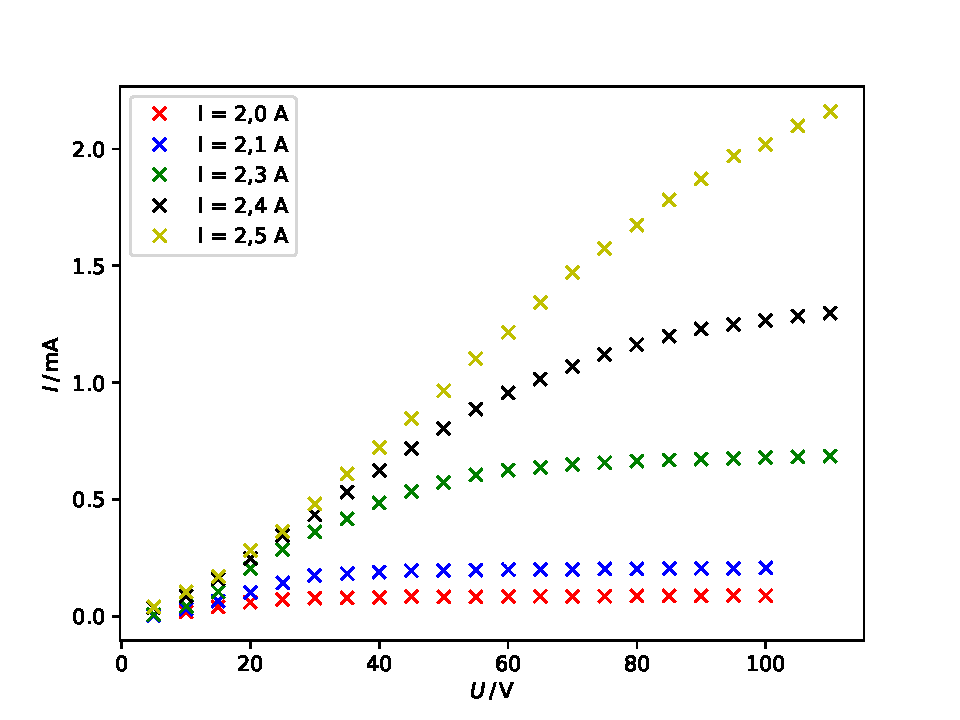
\includegraphics[width=\textwidth]{Plots/kenn.pdf}
  \caption{$U$-$I$-Diagramm mit den fünf Kennlinien}
  \label{fig:kenn}
\end{figure}

Die abgelesenen Sättigungsströme befinden sich in Tabelle \ref{tab:satt}. Für die Heizströme $I_\text{H} = \SI{2,4}{A}$ und $I_\text{H} = \SI{2,5}{A}$
lässt sich kein Sättigungsstrom ablesen.
\begin{table}[H]
   \centering
   \caption{Abgelesene Sättigungsströme}
   \label{tab:satt}
   \begin{tabular} { S S }
 \toprule
 {$I_\text{H}\:/\: \mathrm{A}$} & {$I_\text{S}\:/\: \mathrm{mA}$} \\
    \midrule
    2,0 & 0,088 \\
    2,1 & 0,207 \\
    2,3 & 0,685 \\
    \bottomrule
  \end{tabular}
\end{table}


\subsection{Bestimmung des Exponenten im Langmuir-Schottkyschen Gesetz für die höchste Heizleistung}

Der Geltungsbereich des Langmuir-Schottkyschen Gesetzes liegt ungefähr zwischen $\SI{0}{\V}$ und $\SI{60}{\V}$.
Die Messwerte aus diesem Bereich werden in Abbildung \ref{fig:fit25} doppellogarithmisch aufgetragen.
\begin{figure}[H]
  \centering
  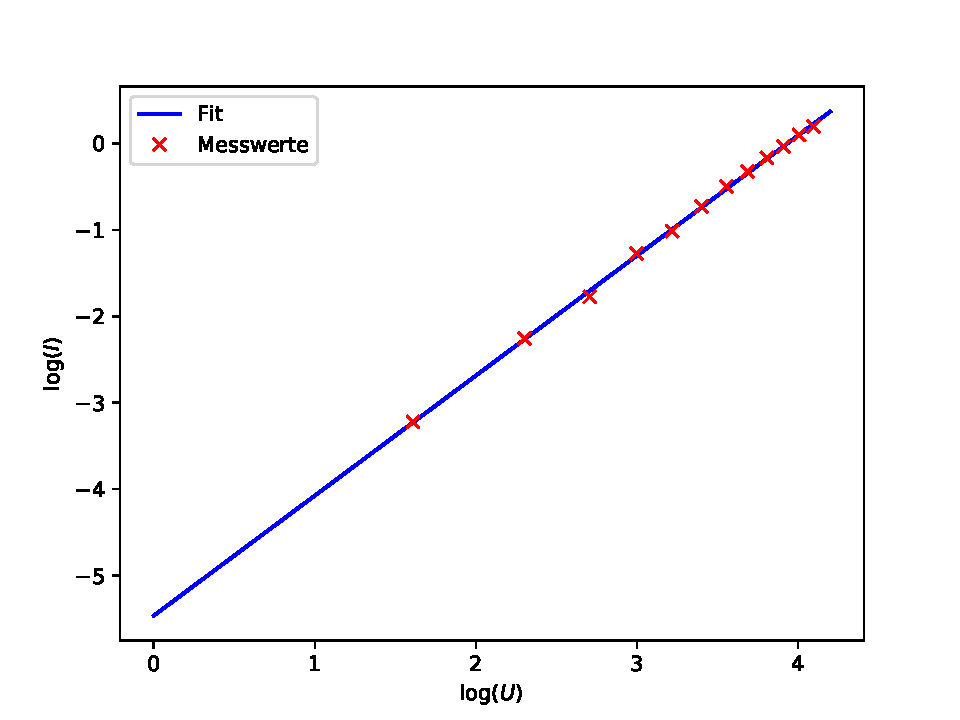
\includegraphics[width=\textwidth]{Plots/fit25.pdf}
  \caption{Doppellogarithmische Darstellung der Kennlinie mit der Heizspannung $I_\text{H} = \SI{2,5}{\V}$}
  \label{fig:fit25}
\end{figure}

Die lineare Regression $f(x) = a \cdot x + b$ liefert die Steigung
\begin{equation*}
  a = 1,39 \pm 0,01
\end{equation*}

Die Abweichung von dem Exponenten in Gleichung \eqref{eqn:LSR} beträgt $7,44 \%$.

\subsection{Bestimmung der Kathodentemperatur über das Anlaufstromgebiet}

Die aufgenommenen Messwerte für den Heizstrom $I_\text{H} = \SI{2,5}{\V}$ befinden sich in Tabelle \ref{tab:anlauf}.
Aufgrund eines nicht funktionierenden Amperemeters wurde der Versuchsaufbau gewechselt.
\begin{table}[H]
   \centering
   \caption{Messwerte für das Anlaufstromgebiet}
   \label{tab:anlauf}
   \begin{tabular} { S S }
 \toprule
 {$U\:/\: \mathrm{V}$} & {$I\:/\: \mathrm{nA}$} \\
    \midrule
    0,00 & 0,900 \\
    0,10 & 0,350 \\
    0,20 & 0,200 \\
    0,26 & 0,150 \\
    0,30 & 0,100 \\
    0,40 & 0,050 \\
    0,42 & 0,020 \\
    0,50 & 0,050 \\
    0,52 & 0,040 \\
    0,60 & 0,020 \\
    0,66 & 0,020 \\
    0,70 & 0,020 \\
    0,74 & 0,012 \\
    0,80 & 0,005 \\
    0,90 & 0,002 \\
    \bottomrule
  \end{tabular}
\end{table}


\newpage
Aufgetragen sind diese in Abbildung \ref{fig:anlauf}.
\begin{figure}[H]
  \centering
  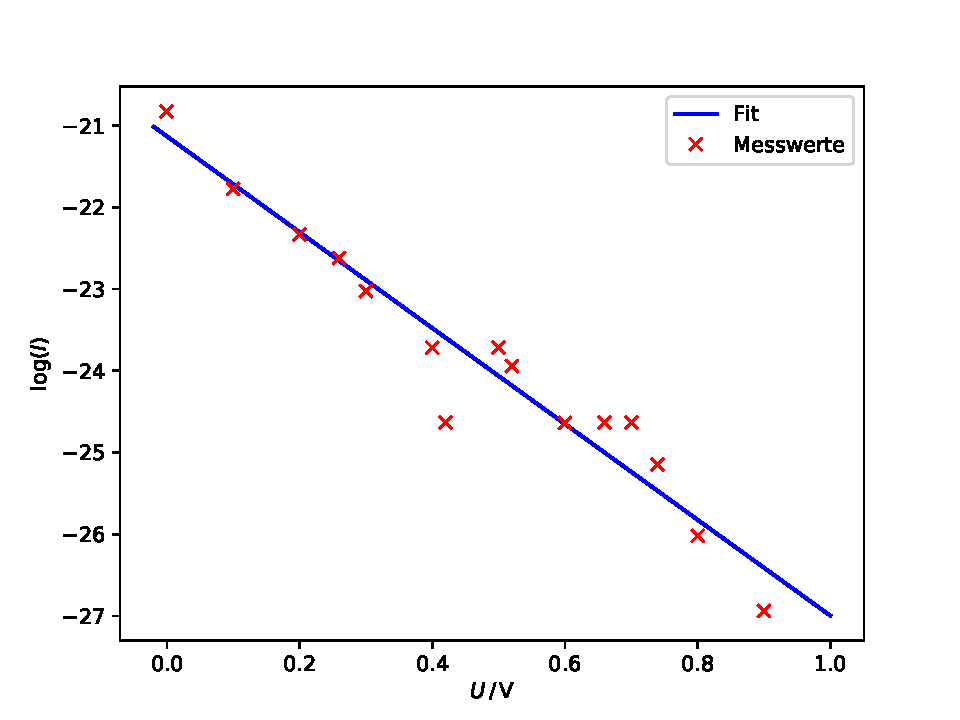
\includegraphics[width=\textwidth]{Plots/anlauf.pdf}
  \caption{Halblogarithmische Auftragung der Messwerte für das Anlaufstromgebiet}
  \label{fig:anlauf}
\end{figure}

Mithilfe der linearen Regression $f(x) = a \cdot x + b$ und der Formel
\begin{equation}
  T = - \frac{e_0 V}{k a}
\end{equation}

ergibt sich eine Kathodentemperatur von $T = \SI{1979,09(14436)}{\K}$.

Der Fehler ergibt sich aus der Gauß'schen Fehlerfortpflanzung
\begin{equation}
  \delta = \sqrt{ \sum_{i=1}^{n}(\frac{\partial y}{\partial x_i} \Delta x_i)^2}.
\end{equation}

\subsection{Bestimmung der Kathodentemperatur mithilfe der Heizleistung}

Die Kathodentemperaturen ergeben sich aus
\begin{equation}
  T = \sqrt[4]{\frac{I U - N_\text{WL}}{f \eta \sigma}}
\end{equation}

und befinden sich in Tabelle \ref{tab:temp}.
Die Wärmeleitung der Diode $N_\text{WL}$ wir dafür als $\SI{1}{\W}$ angenommen. Die restlichen Werte werden der Versuchsanleitung entnommen.
\begin{table}[H]
   \centering
   \caption{Kathodentemperaturen in Abhängigkeit von der Heizleistung}
   \label{tab:temp}
   \begin{tabular} { S S S }
 \toprule
 {$I_\text{H}\:/\: \mathrm{A}$} & {$U_\text{H}\:/\: \mathrm{V}$} & {$T\:/\: \mathrm{K}$} \\
    \midrule
    2,0 & 3,5 & 1851,37 \\
    2,1 & 4,1 & 1964,72 \\
    2,3 & 4,7 & 2093,49 \\
    2,4 & 5,2 & 2177,41 \\
    2,5 & 5,6 & 2246,16 \\
    \bottomrule
  \end{tabular}
\end{table}


\subsection{Berechnung der Austrittarbeit}
Gleichung \eqref{eqn:Anlaufstromstärke} wird nach $\varphi$ umgestellt:
\begin{equation}
  \varphi = - \frac{k T}{e_0} \log{\left( \frac{I_\text{S} h^3}{4 \pi e_0 m_0 f k^2 T^2} \right)}
\end{equation}

Mit den zuvor abgelesenen Sättigungsströmen und den berechneten Kathodentemperaturen ergeben sich die in Tabelle \ref{tab:austritt}
befindlichen Austrittsarbeiten.
\begin{table}[H]
   \centering
   \caption{Austrittsarbeite in Abhängigkeit von der Heizleistung}
   \label{tab:austritt}
   \begin{tabular} { S S }
 \toprule
 {$I_\text{H}\:/\: \mathrm{A}$} & {$\varphi\:/\: \mathrm{eV}$} \\
    \midrule
    2,0 & 4,84 \\
    2,1 & 5,01 \\
    2,3 & 5,13 \\
    \bottomrule
  \end{tabular}
\end{table}


Im Mittel ergibt sich eine Austrittarbeit von $\varphi = \SI{5,00(9)}{\electronvolt}$

Der Mittelwert und die Standardabweichung errechnet sich aus den Gleichungen \eqref{eqn:mit} und \eqref{eqn:sta}.
\begin{equation}
  \bar{x} = \frac{1}{N} \sum_{i=1}^{N} x_i
  \label{eqn:mit}
\end{equation}
\begin{equation}
  \Delta \bar{x} = \sqrt{\frac{1}{N (N - 1)} \sum_{i=1}^{N} (x_i - \bar{x})^2}.
  \label{eqn:sta}
\end{equation}

Der Literaturwert beträgt für Wolfram $\SI{4,54}{\electronvolt}$ \cite{sample2}. Der gemittelte Wert weicht um $10,12 \%$ ab.
